\section{(40점) Compilation Process}

\subsection{Preprocessing}

\begin{enumerate}[label= (\alph*)]
    \item {
        \texttt{cpp -v /dev/null} 명령어를 수행한 결과, 다음과 같은 출력을 얻을 수 있었다.

        \begin{verbatim}
    #include "..." search starts here:
    #include <...> search starts here:
    /usr/lib/gcc/x86_64-linux-gnu/9/include
    /usr/local/include
    /usr/include/x86_64-linux-gnu
    /usr/include
        \end{verbatim}

        이 정보를 바탕으로 첫 번째 디렉토리에서 네 번째 디렉토리까지 \texttt{find} 명령어를 사용하여
        \texttt{stdio.h}, \texttt{math.h} 파일을 검색했다.
        \texttt{stdio.h} 파일의 경우 세 번째 디렉토리인 \texttt{/usr/include/x86\_64-linux-gnu} 에서
        \texttt{find} 명령어가 해당 파일을 찾아내었다.

        \begin{verbatim}
    $ find /usr/include/x86_64-linux-gnu -name "stdio.h"
    /usr/include/x86_64-linux-gnu/bits/stdio.h
        \end{verbatim}

        하지만 찾던 디렉토리에 바로 존재하지 않고, \texttt{bits} 폴더로 한번 더 들어가야
        \texttt{stdio.h} 파일이 존재한다. 따라서 \texttt{cpp}는 이 파일을 찾지 못하고, 사용하지 않는다.

        네 번째 디렉토리인 \texttt{/usr/include} 에서는 디렉토리 바로 아래의 두 파일을 찾을 수 있었다.

        \begin{verbatim}
    $ find /usr/include -name "stdio.h"
    /usr/include/stdio.h
    /usr/include/x86_64-linux-gnu/bits/stdio.h
    /usr/include/c++/9/tr1/stdio.h
    
    $ find /usr/include -name "math.h"
    /usr/include/ucs/sys/math.h
    /usr/include/math.h
    /usr/include/c++/9/tr1/math.h
    /usr/include/c++/9/math.h
        \end{verbatim}

        즉 컴파일러는 각각 \texttt{/usr/include/stdio.h}, \texttt{/usr/include/math.h} 두 파일을 사용한다.
        이는 cpp를 통해 실제 소스코드로 대체된 코드를 직접 살펴보아도 확인할 수 있다[Fig.~\ref{fig:included}].
        각 파일의 라인 수는 875, 1341 이다[Fig.~\ref{fig:1-1_linenum}].

        \begin{figure}
            \centering
            \begin{subfigure}[b]{0.48\textwidth}
                \centering
                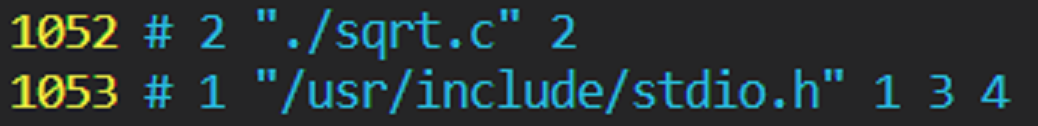
\includegraphics[width=\textwidth]{imgs/Figure00_stdio.png}
                \caption{\texttt{cpp} 가 \texttt{/usr/include/stdio.h}를 사용한 모습.}
                \label{fig:stdio_included}
            \end{subfigure}
            \hfill
            \begin{subfigure}[b]{0.48\textwidth}
                \centering
                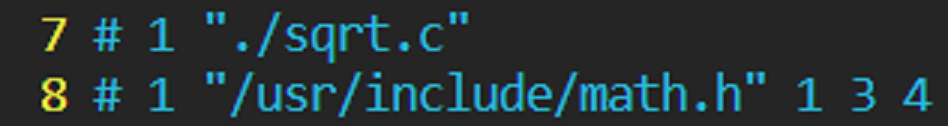
\includegraphics[width=\textwidth]{imgs/Figure00_math.png}
                \caption{\texttt{cpp} 가 \texttt{/usr/include/math.h}를 사용한 모습.}
                \label{fig:math_included}
            \end{subfigure}
            \caption{
                \texttt{cpp}의 preprocess 결과를 통한 검증.
            }
            \label{fig:included}
        \end{figure}
        
        \begin{figure}
            \centering
            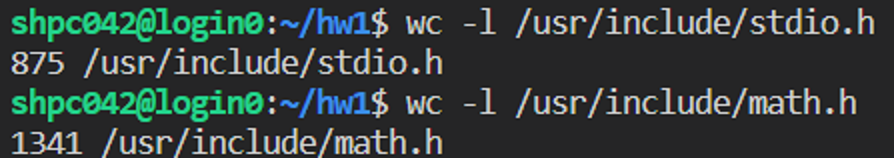
\includegraphics[scale=0.66]{imgs/Figure01_real.png}
            \caption{\label{fig:1-1_linenum}
                \texttt{/usr/include/stdio.h}, \texttt{/usr/include/math.h}
                파일의 라인 수를 출력한 모습.
            }
        \end{figure}
    }

    \item {
        Preprocess까지만 진행하는 \texttt{gcc} 옵션은 \texttt{-E} 이다.
        출력 결과 중 \texttt{scanf}, \texttt{printf}, \texttt{sqrt}를 Fig.~\ref{fig:1-2}와 같이 찾을 수 있었다.

        \begin{figure}[t]
            \centering
            \begin{subfigure}[t]{0.48\textwidth}
                \centering
                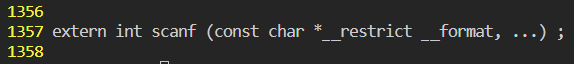
\includegraphics[width=\textwidth]{imgs/Figure02_scanf.png}
                \caption{\texttt{scanf}}
                \label{fig:scanf declaration}
            \end{subfigure}
            \hfill
            \begin{subfigure}[t]{0.48\textwidth}
                \centering
                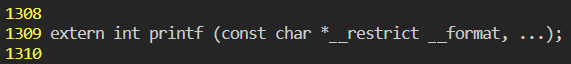
\includegraphics[width=\textwidth]{imgs/Figure03_printf.png}
                \caption{printf}
                \label{fig:printf declaration}
            \end{subfigure}
            \hfill
            \begin{subfigure}[t]{\textwidth}
                \centering
                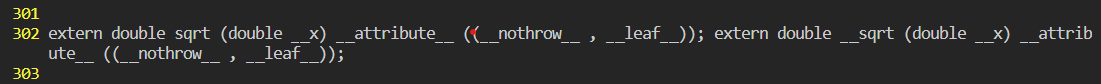
\includegraphics[width=\textwidth]{imgs/Figure04_sqrt.png}
                \caption{sqrt}
                \label{fig:sqrt declaration}
            \end{subfigure}
            \caption{
                Preprocess된 출력 결과 중 \texttt{scanf}, \texttt{printf}, \texttt{sqrt}
                에 대한 부분
            }
            \label{fig:1-2}
       \end{figure}
    }

    \item {
        실제 구현이 들어있지 않다. \texttt{sqrt.c} 파일에서 참조한 파일들은 헤더 파일(\texttt{.h})로,
        보통 함수를 선언하는 코드로 채운다. 같은 헤더 파일을 공유함으로서 같은 심볼에 대해 같은 선언을 기반으로
        컴파일할 수 있게 하기 위함이다. 실제 구현은 별도의 오브젝트 파일(\texttt{.o}) 또는
        공유 오브젝트 파일(\texttt{.so}) 속에 준비되어 있으며, 링킹 과정에서 합쳐진다.
    }
    
\end{enumerate}

\subsection{Compilation}

\begin{enumerate}[label= (\alph*)]
    \item {
        Object file을 출력하는 \texttt{gcc} 옵션은 \texttt{-c} 이다.
        다음과 같은 명령어를 사용할 수 있다.

        \begin{verbatim}
    $ gcc -c sqrt.c
        \end{verbatim}
    }

    \item {
        Linux 운영체제에서는 파일을 다음과 같이 총 7가지로 분류한다.
        
        \begin{itemize}
            \item Regular files
            \item Directories
            \item Character device files
            \item Block device files
            \item Local domain sockets
            \item Named pipes (FIFOs)
            \item Symbolic links
        \end{itemize}
        
        파일이 이 중 어디에 속하는지는 \texttt{stat} 명령어를 사용하여 알아낼 수 있다.

        \begin{verbatim}
    $ stat -c "%F" sqrt.o
    regular file
        \end{verbatim}

        즉 sqrt.o 파일은 Linux 운영체제의 파일 분류 중 regular file에 해당한다.

        추가로, Linux 파일에서는 magic number라는 시스템을 사용한다. 이는 파일의 최초 2바이트 영역에
        저장되는 숫자를 말하며, 파일의 타입에 대한 간단한 메타데이터를 제공하는 역할을 한다.
        \texttt{file} 명령어를 사용하여 파일의 magic number로부터 파일에 대한 정보를 얻을 수 있다.

        \begin{verbatim}
    $ file sqrt.o
    sqrt.o: ELF 64-bit LSB relocatable, x86-64, version 1 (SYSV), not stripped
        \end{verbatim}
    }
    
\end{enumerate}

\subsection{Linking}

\begin{enumerate}[label= (\alph*)]
    \item {
        \texttt{sqrt} 함수에 대한 구현 부분이 컴파일 과정에 제공되지 않았기 때문에 링킹 과정에서
        에러가 발생하였다.
        올바르게 컴파일하기 위해서는 \texttt{sqrt} 함수에 대한 구현이 포함된 오브젝트 파일을
        \texttt{-lm} 명령어를 통해 제공해야 한다. 결과적으로 다음과 같은 명령어를 통해
        올바르게 컴파일할 수 있다.

        \begin{verbatim}
    $ gcc sqrt.o -lm
        \end{verbatim}
    }

    \item {
        Fig.~\ref{fig:1-3}과 같이 \texttt{sqrt} 함수를 실행해보았다.

        \begin{figure}
            \centering
            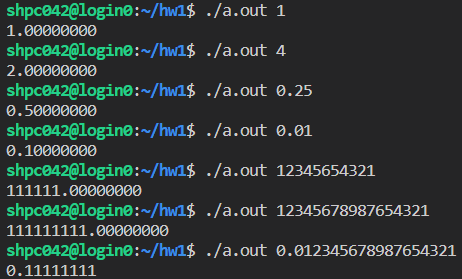
\includegraphics[scale=1]{imgs/Figure05_sqrt_trial.png}
            \caption{\label{fig:1-3}
                \texttt{sqrt}에 임의의 수를 입력한 결과.
            }
        \end{figure}
    }
    
\end{enumerate}